\documentclass[11pt]{article}
\usepackage[margin=1in]{geometry}
\usepackage{amsmath,amssymb,graphicx,booktabs,hyperref,longtable}
\title{MIZN run report: \texttt{cara_default}}
\author{auto-generated}
\date{2026-06-20T09:28:27.291376+00:00}

\begin{document}\maketitle

\section*{1.~Summary}
Scenario \texttt{cara_default} on model \texttt{cara},
grid \texttt{u},
step2 \texttt{gaussian},
solver \texttt{picard}.
Converged in 1 iterations to $\|F\|_\infty = 6.853e-18$
in 0.00\,s.

\section*{2.~Configuration}
\begin{tabular}{ll}\toprule
parameter & value \\\midrule
\texttt{tau\_th} & 1.0 \\
\texttt{tau\_eps} & 2.0 \\
\texttt{tau\_u} & 1.0 \\
\texttt{rho} & 2.0 \\
\texttt{gamma} & 2.0 \\
\texttt{theta\_bar} & 0.0 \\
\texttt{u\_bar} & 0.0 \\
\texttt{G} & 9 \\
\texttt{umax} & 4.0 \\
\texttt{model} & cara \\
\texttt{grid} & u \\
\texttt{step2} & gaussian \\
\texttt{solver} & picard \\
\texttt{tol} & 1e-12 \\
\texttt{maxit} & 200 \\
\texttt{omega} & 0.5 \\
\texttt{anderson\_m} & 8 \\
\bottomrule
\end{tabular}

\section*{3.~Result metrics}
\begin{tabular}{lr}\toprule
metric & value \\\midrule
$\|F\|_\infty$              & 6.853e-18 \\
slope$_T$                    & 0.75000 \\
deficit ($1-R^2$)            & 0.00000e+00 \\
$d_\mathrm{FR}$              & 2.0412 \\
$\max|P-P_\mathrm{analytic}|$ & 3.427e-18 \\
iterations                   & 1 \\
walltime (s)                 & 0.00 \\
\bottomrule
\end{tabular}

\section*{4.~Convergence}
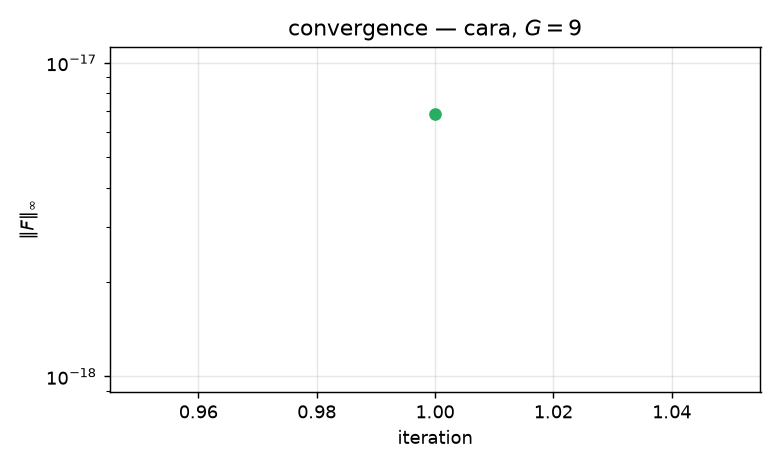
\includegraphics[width=\linewidth]{artifacts/plots/convergence.png}

\section*{5.~Fixed point}
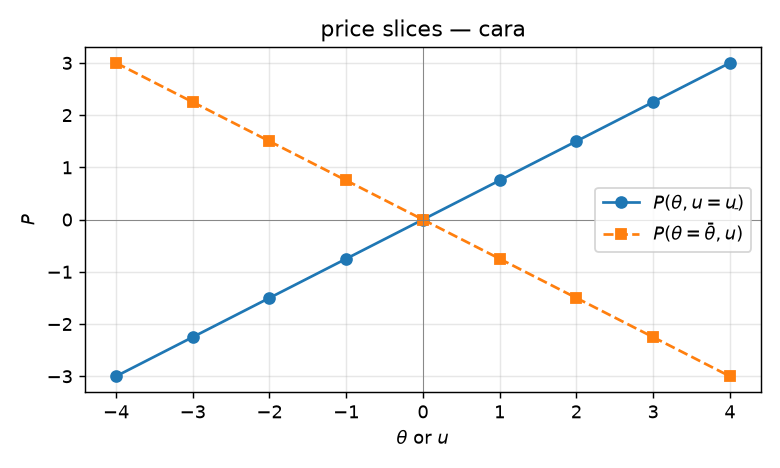
\includegraphics[width=\linewidth]{artifacts/plots/P_slices.png}

\section*{6.~Version manifest}
\small\begin{longtable}{lll}\toprule
file & git\_blob (first 10) & sha256 (first 10) \\\midrule
\texttt{src/mizn/\_\_init\_\_.py} & \texttt{396e69e9f1} & \texttt{baece35fe8} \\
\texttt{src/mizn/analytic.py} & \texttt{3ef97dcc65} & \texttt{719c59877a} \\
\texttt{src/mizn/config.py} & \texttt{f58f7ec60e} & \texttt{302495e2a2} \\
\texttt{src/mizn/diagnostics/\_\_init\_\_.py} & \texttt{5033c93115} & \texttt{cf774e4e44} \\
\texttt{src/mizn/diagnostics/metrics.py} & \texttt{95b9a86b71} & \texttt{98be50a1fc} \\
\texttt{src/mizn/diagnostics/plotting.py} & \texttt{51fb6cbbd3} & \texttt{2a7f641316} \\
\texttt{src/mizn/grid/\_\_init\_\_.py} & \texttt{2bc9aebdc2} & \texttt{ae3b0e96b6} \\
\texttt{src/mizn/grid/base.py} & \texttt{dd1096378b} & \texttt{a85efb4094} \\
\texttt{src/mizn/grid/linear\_u.py} & \texttt{6a4b715cd4} & \texttt{d07849e7bc} \\
\texttt{src/mizn/main.py} & \texttt{8ee4ac410f} & \texttt{f78f3f6785} \\
\texttt{src/mizn/signals.py} & \texttt{9f16ff2362} & \texttt{9745638ad0} \\
\texttt{src/mizn/solvers/\_\_init\_\_.py} & \texttt{3fee61d2d6} & \texttt{8201e8eaf1} \\
\texttt{src/mizn/solvers/picard.py} & \texttt{f2435eadda} & \texttt{667fa67acd} \\
\texttt{src/mizn/step1\_conjecture.py} & \texttt{542a59025f} & \texttt{bf596cd6be} \\
\texttt{src/mizn/step2\_learning/\_\_init\_\_.py} & \texttt{ef694c1200} & \texttt{743d26473e} \\
\texttt{src/mizn/step2\_learning/gaussian.py} & \texttt{55acff23be} & \texttt{7db517ce4f} \\
\texttt{src/mizn/step3\_demand/\_\_init\_\_.py} & \texttt{2d5c3f3b9e} & \texttt{7ed74e98ad} \\
\texttt{src/mizn/step3\_demand/cara.py} & \texttt{7166e7db11} & \texttt{42250729e6} \\
\texttt{src/mizn/step4\_aggregate.py} & \texttt{41990ce1c7} & \texttt{ab7da6edc2} \\
\texttt{src/mizn/step5\_clearing/\_\_init\_\_.py} & \texttt{1a5bfbb453} & \texttt{15eb3e529c} \\
\texttt{src/mizn/step5\_clearing/cara.py} & \texttt{e6f0c3d569} & \texttt{68359fe7af} \\
\bottomrule
\end{longtable}

Active variants:
\texttt{model=cara, grid=u,
        step2=gaussian, solver=picard}.\\
Repo SHA: \texttt{ 06d6aa5475 }
(DIRTY).

\section*{7.~Notes (manual)}
\IfFileExists{notes.tex}{\input{notes.tex}}{(none)}

\end{document}